\documentclass[fleqn]{article}

%\pgfplotsset{compat=1.17}

\usepackage{mathexam}
\usepackage{amsmath}
\usepackage{amsfonts}
\usepackage{graphicx}
\usepackage{systeme}
\usepackage{microtype}
\usepackage{multirow}
\usepackage{pgfplots}
\usepackage{listings}
\usepackage{tikz}
\usepackage{dsfont} %Numeros reales, naturales...
\usepackage{cancel}

%\graphicspath{{images/}}
\newcommand*{\QED}{\hfill\ensuremath{\square}}

%Estructura de ecuaciones
\setlength{\textwidth}{15cm} \setlength{\oddsidemargin}{5mm}
\setlength{\textheight}{23cm} \setlength{\topmargin}{-1cm}



\author{David García Curbelo}
\title{Ecuaciones}

\pagestyle{empty}


\def\R{\mathds{R}}
\def\Z{\mathds{Z}}
\def\N{\mathds{N}}

\def\sup{$^2$}

\def\next{\quad \Rightarrow \quad}

\begin{document}
    \maketitle
    \setcounter{page}{1}
    \pagestyle{plain}

    \textbf{Ejercicio 1. } \\

    No es relevante que dos superficies sean difeomorfas para que tengan la misma imagen esférica. Sabemos que ambas superficies (el cilindro elíptico y el catenoide) 
    son superficies difeomorfas, y además ambas son orientables. Por ser orientables podemos cosniderar una orientación para cada una de las superficies, y por tanto una aplicación 
    de Gauss para cada una de ellas, dada por 
    \begin{equation*}
        N_1: S_1 \longrightarrow \mathds{S}^2\\
        N_2: S_2 \longrightarrow \mathds{S}^2
    \end{equation*}
    siendo $S_1$ y $S_2$ el cilindro y el catenoide, respectivamente. Calculemos primero la imagen esférica del cilindro. para ello consideramos el conjunto
    $$S_1 = \{\alpha(t) + v\vec{e}_3 \thinspace : \thinspace t\in I, \thinspace v\in \R\}$$
    Donde $\alpha(t)$ viene dado por la elipse $\alpha(t) = (a\cos(t), b\sin(t), 0), \thinspace a,b\in \R$. Consideremos por tanto la siguiente parametrización, en la que nos basaremos para 
    la construcción de $N_1$.
    \begin{equation*}
        \begin{aligned}
            & F:\R^2 \rightarrow S_1 \subset \R^3 \\
            &F(t,v) = (a\cos(t), b\sin(t), v)
        \end{aligned}
    \end{equation*}
    Y realizando los siguientes cálculos
    \begin{equation*}
        F_t = (-a\sin(t), b\cos(t), 0) \\
        F_v = (0,0,1) \\
        F_t \times F_v = (b\cos(t), a\sin(t), 0)
    \end{equation*}
    obtenemos fácilmente la fórmula de Gauss:
    $$N_1(F(t,v)) = \frac{F_t \times F_v}{\left|F_t \times F_v\right|} = \frac{1}{\sqrt{a^2\sin^2(t) + b^2\cos^2(t)}} (b\cos(t), a\sin(t), 0)$$
    Donde podemos observar que dicha aplicación de Gauss lleva cualquier cilindro elíptico a la circunferencia obtenida de intersecar la esfera $\mathds{S}^2$ con el plano $z=0$. Calculemos
    ahora la aplicación de Gauss para el catenoide. Sabemos que se trata de una superficie de revolución, al rotar (en este caso) sobre el eje $z$ una catenaria de la forma
    $\alpha(t) = (a\cosh(t), 0, bt), \thinspace \thinspace a,b\in \R-\{0\}$. Por ello, obtengamos la imagen esférica del campo normal unitario de nuestra catenaria (que será nuestra curva generatriz),
    la cual rotaremos posteriormente para obtener así la imagen esférica de toda la superficie. Para ello consideremos su referencia de Frenet, la cual viene dada por
    $$N(t) = \left(\frac{\sinh(t)}{\cosh(t)}, 0, \frac{1}{\cosh(t)} \right)$$
    Con la que podemos ver que se trata de una semicircunferencia sin los extremos, y que por tanto al rotarla obtenemos
    que la imagen esférica del catenoide es toda la esfera $\mathds{S}^2$ sin las antípodas que pasan por el eje $z$, es decir, $\mathds{S}^2 - \{(0,0,1), (0,0,-1)\}$, y por tanto podemos ver que,
    a pesar de ser dos superficies difeomorfas, poseen imágenes esféricas distintas.\\ \\

    \textbf{Ejercicio 2. } \\

    El enunciado mencionado es claramente falso. Nos encontramos ante una doble implicación, en la que la implicación hacia la izquierda sabemos que es cierto por un resultado 
    visto en clase, pero el recíproco no es siempre cierto. Para ello consideremos el siguiente contraejemplo:

    Partamos de la hipótesis de que nos encontramos en una superficie $S$ para la cual vamos a considerar $S=\mathds{S}^2$ la esfera unidad de radio 1 y centrada en el origen. 
    Conideremos también un punto de la superficie $p_0 = (1,0,0)$, y tomemos la siguiente parametrización que cubra a dicho punto
    \begin{equation*}
        X: I\times \R \longrightarrow \mathds{S}^2 \subset \R^3 \\
        X(u,v) = \left(\sqrt{1-u^2-v^2}, u, v\right)
    \end{equation*} 
    Con la cual calculamos ahora las bases del plano tangente, que vienen dadas por
    \begin{equation*}
        X_u = \left(\frac{-u}{\sqrt{1-u^2-v^2}}, 1, 0\right) \\
        X_v = \left(\frac{-v}{\sqrt{1-u^2-v^2}}, 0, 1\right)    
    \end{equation*}
    Y calculemos con ella la función curvatura de Gauss, que viene dada por la siguiente fórmula
    \begin{equation*}
        X_u \times X_v = \left(1, \frac{u}{\sqrt{1-u^2-v^2}}, \frac{v}{\sqrt{1-u^2-v^2}}\right), \quad\\
        N(X(u,v)) = \frac{X_u \times X_v}{|X_u \times X_v|} = \left(\sqrt{1-u^2-v^2}, u, v\right)
    \end{equation*}
    Ahora que tenemos todas las herramientas, vamos a definir dos curvas $\alpha(t)$ y $\beta(t)$ tales que cumplan las siguientes condiciones
    \begin{equation*}
        \alpha(0) = \beta(0) = p_0 = (1,0,0) \\
        \alpha'(0) = (0,1,0) \\
        \beta' (0) = (0,0,1)
    \end{equation*}
    Por tanto, en estas condiciones podemos ver que nos entcontramos ante una superficie en la que tenemos dos curvas que se cortan, cuya curvatura normal es la misma en el 
    punto de intersección, $N(\alpha(0)) = N(\beta(0)) = (1,0,0)$, pero cuyas tangentes hemos visto que son distintas, por lo que el enunciado dado no es cierto.

    \textbf{Ejercicio 3. } \\

    Para poder comprobar la veracidad o falsedad del enunciado, necesitamos saber la función curvatura de Gauss en toda la superficie, para poder así clasificar sus puntos. Sabemos que el 
    toro elíptico es una superficie de revolución resultado de rotar con respecto al eje $z$ la curva $\alpha(t) = (R + a\cos(t), 0, b\sin(t))$, donde $R>a, \thinspace a \neq b$. Sabiendo esto,
    podemos definir la matriz del operador forma como sigue 
    $$A=
    \begin{pmatrix}
        k(t) & 0 \\
        0 & \frac{\alpha_3'(t)}{\alpha_1(t) |\alpha'(t)|}
    \end{pmatrix}
    $$
    por ser una superficie de revolución, donde $k(t)$ es la curvatura de la curva $\alpha(t)$, la cual sabemos que viene dada por $k(t)=\frac{ab}{(a^2\sin^2(t) + b^2 \cos^2(t))^{\frac{3}{2}}}$, que además es positiva
    para todo $t\in \R$. Por ello, como sabemos que las función de curvatura de Gauss viene dada por el producto de los valores propios de dicha matriz (o lo que es lo mismo, por su determinante), vemos que
    $$K = \frac{ab}{(a^2\sin^2(t) + b^2 \cos^2(t))^{\frac{3}{2}}} \frac{\alpha_3'(t)}{\alpha_1(t)} = \frac{ab^2 \cos(t)}{(R + a\cos(t))(a^2\sin^2(t) + b^2 \cos^2(t))^{\frac{3}{2}}}$$
    Estudiando el signo de dicha igualdad, observamos que cuando $t=\frac{\pi}{2}$ ó $t=-\frac{\pi}{2}$, tenemos que $K=0$, por lo que los paralelos generados al girar estos dos puntos
    de la curva $\alpha(t)$ están compuestos por puntos parabólicos. Por ello podemos concluir que un toro elíptico NO tiene todos sus puntos elípticos, ya que contiene otros 
    tipos de puntos. \\ \\

    \newpage

    \textbf{Ejercicio 4. } \\
   
    Calculemos primero sus curvaturas. Para ello definamos primero la función siguiente
    \begin{equation*}
        \begin{aligned}
            & F:\R^2 \rightarrow C_{\alpha} \subset \R^3 \\
            &F(t,v) = (t, 2\cosh(t), v)
        \end{aligned}
    \end{equation*}
    siendo $C_{\alpha}$ la superficie que queremos estudiar. Consideremos a continuación la matriz asociada al operador forma del cilindro que estamos estudiando, 
    la cual viene dada por
    \begin{equation*}
        A =
        \begin{pmatrix}
            a_{11} & a_{12} \\
            a_{21} & a_{22}
        \end{pmatrix}
        = \frac{1}{\langle F_t, F_t \rangle \langle F_v, F_v \rangle - \langle F_t, F_v \rangle ^2}
        \begin{pmatrix}
            \langle F_v, F_v \rangle & - \langle F_t, F_v \rangle \\
            -\langle F_t, F_v \rangle & \langle F_t, F_t \rangle
        \end{pmatrix}
        \begin{pmatrix}
            \langle F_{tt}, N \rangle & \langle F_{tv}, N \rangle \\
            \langle F_{vt}, N \rangle & \langle F_{vv}, N \rangle
        \end{pmatrix}
    \end{equation*}
    Donde $F_t$, $F_v$, $F_{tv}$, $F_{vv}$, $F_{vt}$ y $F_{tt}$ vienen dados por
    \begin{equation*}
        F_t = (1, 2\sinh(t), 0) \\
        F_v = (0, 0, 1) \\
        F_{tt} = (0, 2\cosh(t), 0) \\
        F_{tv} = F_{vt} = F_{vv} = (0, 0, 0)
    \end{equation*}
    Y $N$ es la aplicación de Gauss, la cual se calcula de la siguiente manera:
    \begin{equation*}
        F_t \times F_v = (2\sinh(t), -1, 0) \\
        N(F(t,v)) = \frac{F_t \times F_v}{|F_t \times F_v|} = \frac{1}{|\alpha'(t)|} (2\sinh(t), -1, 0)
    \end{equation*}
    Por lo tanto, realizando los productos pertinentes obtenemos la matriz $A$ del operador forma
    \begin{equation*}
        A = \frac{1}{4\sinh^2(t) +1}
        \begin{pmatrix}
            1 & 0\\
            0 & 4\sinh^2(t) +1
        \end{pmatrix}
        \begin{pmatrix}
            -\frac{2\cosh(t)}{|\alpha'(t)|} & 0 \\
            0 & 0
        \end{pmatrix} = 
        \begin{pmatrix}
            -\frac{2\cosh(t)}{|\alpha'(t)|} & 0 \\
            0 & 0
        \end{pmatrix}
    \end{equation*}

    $$\Rightarrow A =
    \begin{pmatrix}
        -\frac{2\cosh(t)}{|\alpha'(t)|} & 0 \\
        0 & 0
    \end{pmatrix}
    $$
    Como bien sabemos, las curvaturas principales vienen dadas por los valores propios de la matriz asociada al operador forma, que en nuestro caso es fácil obtener 
    ya que la matriz se encuentra en su forma diagonal, por lo que tenemos $k_1 = -\frac{2\cosh(t)}{|\alpha'(t)|} $ y $k_2 = 0$. Ahora, para la curvatura de Gauss ($K$) y la curvatura
    media ($H$) basta con considerar el determinante y la traza de la matriz, respectivamente, de la siguiente manera:
    \begin{equation*}
        K = det(A) = k_1 k_2 = 0 \\
        H = \frac{1}{2}(k_1 + k_2) = \frac{1}{2}k_1 = -\frac{\cosh(t)}{|\alpha'(t)|}
    \end{equation*} 

    Para calcular las direcciones principales, basta con ver que nos encontramos en un caso particular, en el que $\langle F_{tv}, N \rangle = \langle F_{t}, F_v \rangle = 0$
    y por tanto tenemos que $F_t$ y $F_v$ son las direcciones principales en cada punto de la parametrización.\\ \\

    \textbf{Ejercicio 5. } \\

    Es verdadero. Basta con ver que un paralelo de una superficie de revolución es el resultado de girar un cierto punto $\alpha(t_0)$ de la curva generatriz de la superficie con respecto
    al eje de giro. Por ello, al clasificar un cierto punto de dicha curva generatriz, que es clasificado mediante la función curvatura de Gauss, vemos que $K$ no depende del ángulo rotado,
    y por tanto la clasificación del punto se mantiene a lo largo del paralelo. 
    
    Como ejemplo podemos considerar el toro elíptico calculado en el \textit{Ejercicio 3}, en el cual vimos que 
    cuando la curva generatriz tomaba el valor $\frac{\pi}{2}$ (y por tanto considerábamos dicho punto $\alpha(\frac{\pi}{2})$), vimos que el valor de la curvatura de Gauss era nula, y concluíamos
    que, tanto dicho punto como todo su paralelo, estaban constituidos por puntos parabólicos. \\ \\

    \textbf{Ejercicio 6. } \\

    Para clasificar los puntos de dicho grafo necesitamos saber el signo de la función curvatura de Gauss, y a partir de ella y de sus curvaturas principales podremos clasificar cualquier punto
    de la superficie dada. Para ello primero tenemos que parametrizar la superficie dada por el grafo $h$, la cual nos queda de la siguiente manera
    \begin{equation*}
        \begin{aligned}
            X: \R^2 &\longrightarrow S \\
            (u,v) &\longrightarrow X(u, v) = (u, v, h(u,v)) = (u, v, u^3 + v^3)
        \end{aligned}
    \end{equation*}
    Para calcular la curvatura de Gauss y clasificar así los puntos, vamos a necesitar calcular primero la matriz asociada al operador forma, la cual viene dada por 
    \begin{equation*}
        A =
        \begin{pmatrix}
            a_{11} & a_{12} \\
            a_{21} & a_{22}
        \end{pmatrix}
        = \frac{1}{\langle X_u, X_u \rangle \langle X_v, X_v \rangle - \langle X_u, X_v \rangle ^2}
        \begin{pmatrix}
            \langle X_v, X_v \rangle & - \langle X_u, X_v \rangle \\
            -\langle X_u, X_v \rangle & \langle X_u, X_u \rangle
        \end{pmatrix}
        \begin{pmatrix}
            \langle X_{uu}, N \rangle & \langle X_{uv}, N \rangle \\
            \langle X_{vu}, N \rangle & \langle X_{vv}, N \rangle
        \end{pmatrix}
    \end{equation*}
    Donde $X_u$, $X_v$, $X_{uv}$, $X_{vv}$, $X_{vu}$ y $X_{uu}$ vienen dados por
    $$
        X_u = (1, 0, 3u^2) \quad \quad \quad \quad
        X_v = (0, 1, 3v^2)
    $$
    $$
        X_{uu} = (0, 0, 6u)\quad \quad \quad \quad
        X_{vv} = (0, 0, 6v)\quad \quad \quad \quad
        X_{uv} = X_{vu} = (0, 0, 0)
    $$
    Y $N$ es la aplicación de Gauss, la cual se calcula de la siguiente manera:
    \begin{equation*}
        X_u \times X_v = (-3u^2, - 3v^2, 1) \\
        N(X(u,v)) = \frac{X_u \times X_v}{|X_u \times X_v|} = \frac{1}{\sqrt{9(u^4 + v^4) + 1}}(-3u^2, - 3v^2, 1)
    \end{equation*}
    Y por tanto, calculando los valores para la resolución de la matriz $A$ tenemos
    $$
    A = \frac{1}{(1 + 9v^4)(1 + 9u^4) - 81(uv)^4}
    \begin{pmatrix}
        1+9v^4 & -9u^2v^2 \\
        -9u^2v^2 & 1+9u^4
    \end{pmatrix}
    \frac{1}{\sqrt{9(u^4 + v^4) + 1}}
    \begin{pmatrix}
        6u & 0 \\
        0 & 6v
    \end{pmatrix}
    $$

    $$
    \Rightarrow A = \frac{6}{(9u^4 + 9v^4 + 1)^{3/2}}
    \begin{pmatrix}
        u(1+9v^4) & -9u^2v^3 \\
        -9u^3v^2 & v(1+9u^4)
    \end{pmatrix}
    $$
    Como bien sabemos, la curvatura de Gauss ($K$) viene dada por el determinante de la matriz $A$ que acabamos de calcular, y por tanto tenemos
    $$K(u,v) = \frac{36uv}{(9u^4 + 9v^4 + 1)^{2}}$$
    Estudiemos por tanto el signo de dicha función y así podremos clasificar sus puntos a lo largo de la superficie. podemos ver en primera instancia que el denominador
    es positivo y distinto de cero $\forall (u,v) \in \R^2$, por lo tanto preocupémonos en estudiar el signo del numerador (el cual nos proporcionará el signo del determinante). 
    Vemos claramente que el determinante se anula cuando al menos uno de los dos parámetros $u$ ó $v$ toma el valor $0$. Consideramos por tanto tres casos a 
    distinguir para estudiar cuando el determinante es nulo:
    \begin{enumerate}
        \item[$u=0, \thinspace v\neq 0$] Sustituyendo en la matriz $A$ podemos ver que resulta una matriz diagonal con un valor propio no nulo, 
                $k_1 = 0$, $k_2 = \frac{6v}{(9v^4 + 1)^{3/2}}$, y por lo tanto todo punto de la forma $(0,v)$ es un punto parabólico.
        \item[$v=0, \thinspace u\neq 0$] Sustituyendo en la matriz $A$ podemos ver que resulta una matriz diagonal con un valor propio no nulo, 
                $k_1 = \frac{6u}{(9v^4 + 1)^{3/2}}$, $k_2 = 0$, y por lo tanto todo punto de la forma $(u,0)$ es un punto parabólico.
        \item[$u = v = 0$] Este es un caso un poco más sutil, ya que al sustituir en la matriz $A$ vemos que la matriz obtenida es una matriz nula, es decir,
                con ambos valores propios nulos, por lo que el punto $(0,0)$ se trata de un punto plano. 
    \end{enumerate}
    Podemos afirmar que en el resto de situaciones el determinante será no nulo, y por ello además sus valores propios serán de la misma forma no nulos.
    Continuando con la clasificación, vemos de manera sencilla que cuando ambos parámetros se encunetren en una de las dos siguientes situaciones, 
    \begin{equation*}
        v>0, \thinspace u<0 \\
        u>0, \thinspace v<0
    \end{equation*}
    la curvatura de Gauss será de signo negativo, y entonces nos encontraremos ante un punto hiperbólico. De forma similar podemos ver que cuando ambos parámetros 
    tengan el mismo signo, es decir, en los casos
    \begin{equation*}
        u>0, \thinspace v>0 \\
        u<0, \thinspace v<0
    \end{equation*}
    el valor de la curvatura de Gauss será positiva, y por tanto dicho punto será elíptico. En resumen:
    \begin{itemize}
        \item Punto plano: $(u,v) = (0,0)$
        \item Punto parabólico: $(u,v) \in \{(x,y)/ \quad xy=0, \thinspace (x,y)\neq (0,0)\}$ 
        \item Punto elíptico: $(u,v) \in \thinspace \{\R^+ \times \R^+\} \cup \{\R^- \times \R^-\}$
        \item Punto hiperbólico: $(u,v) \in \thinspace \{\R^+ \times \R^-\} \cup \{\R^- \times \R^+\}$
    \end{itemize}
    \begin{figure}
        \centering
        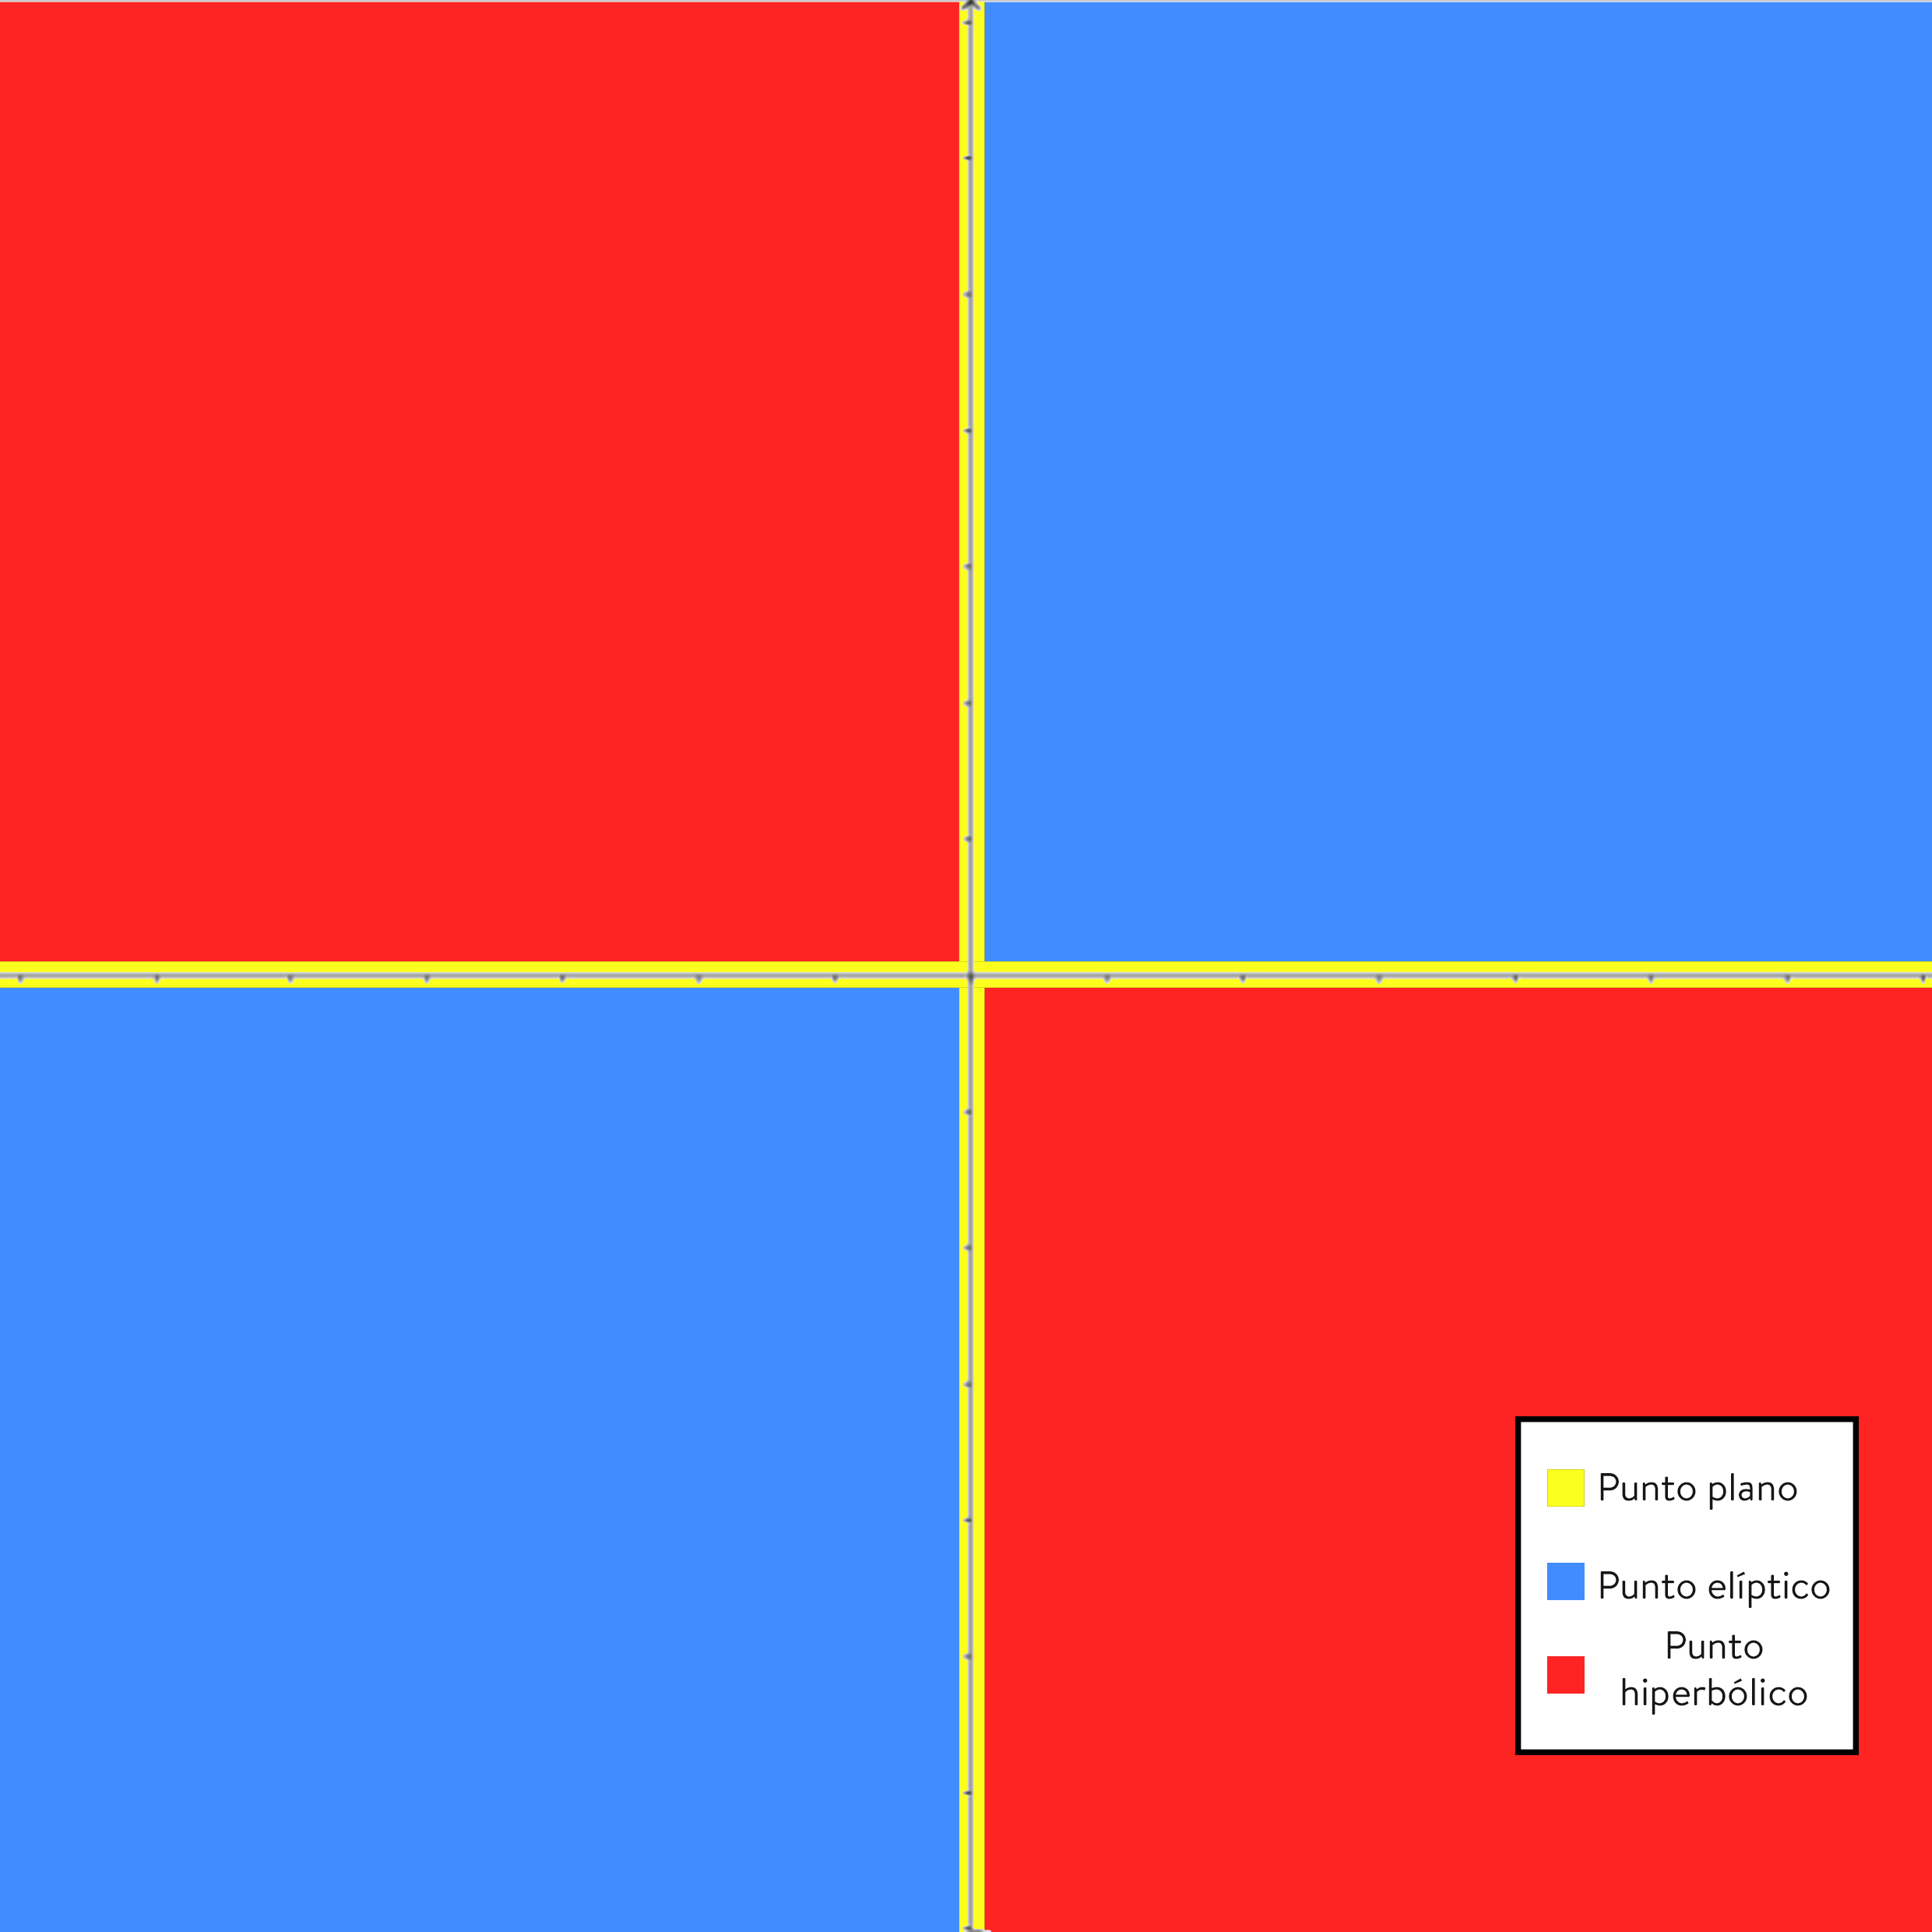
\includegraphics[scale = 0.2]{grafica.png}
        \caption{Distribución de puntos en el plano}
    \end{figure}
\end{document}